\begin{figure}[htb!]
\centering
\begin{tabular}{c}
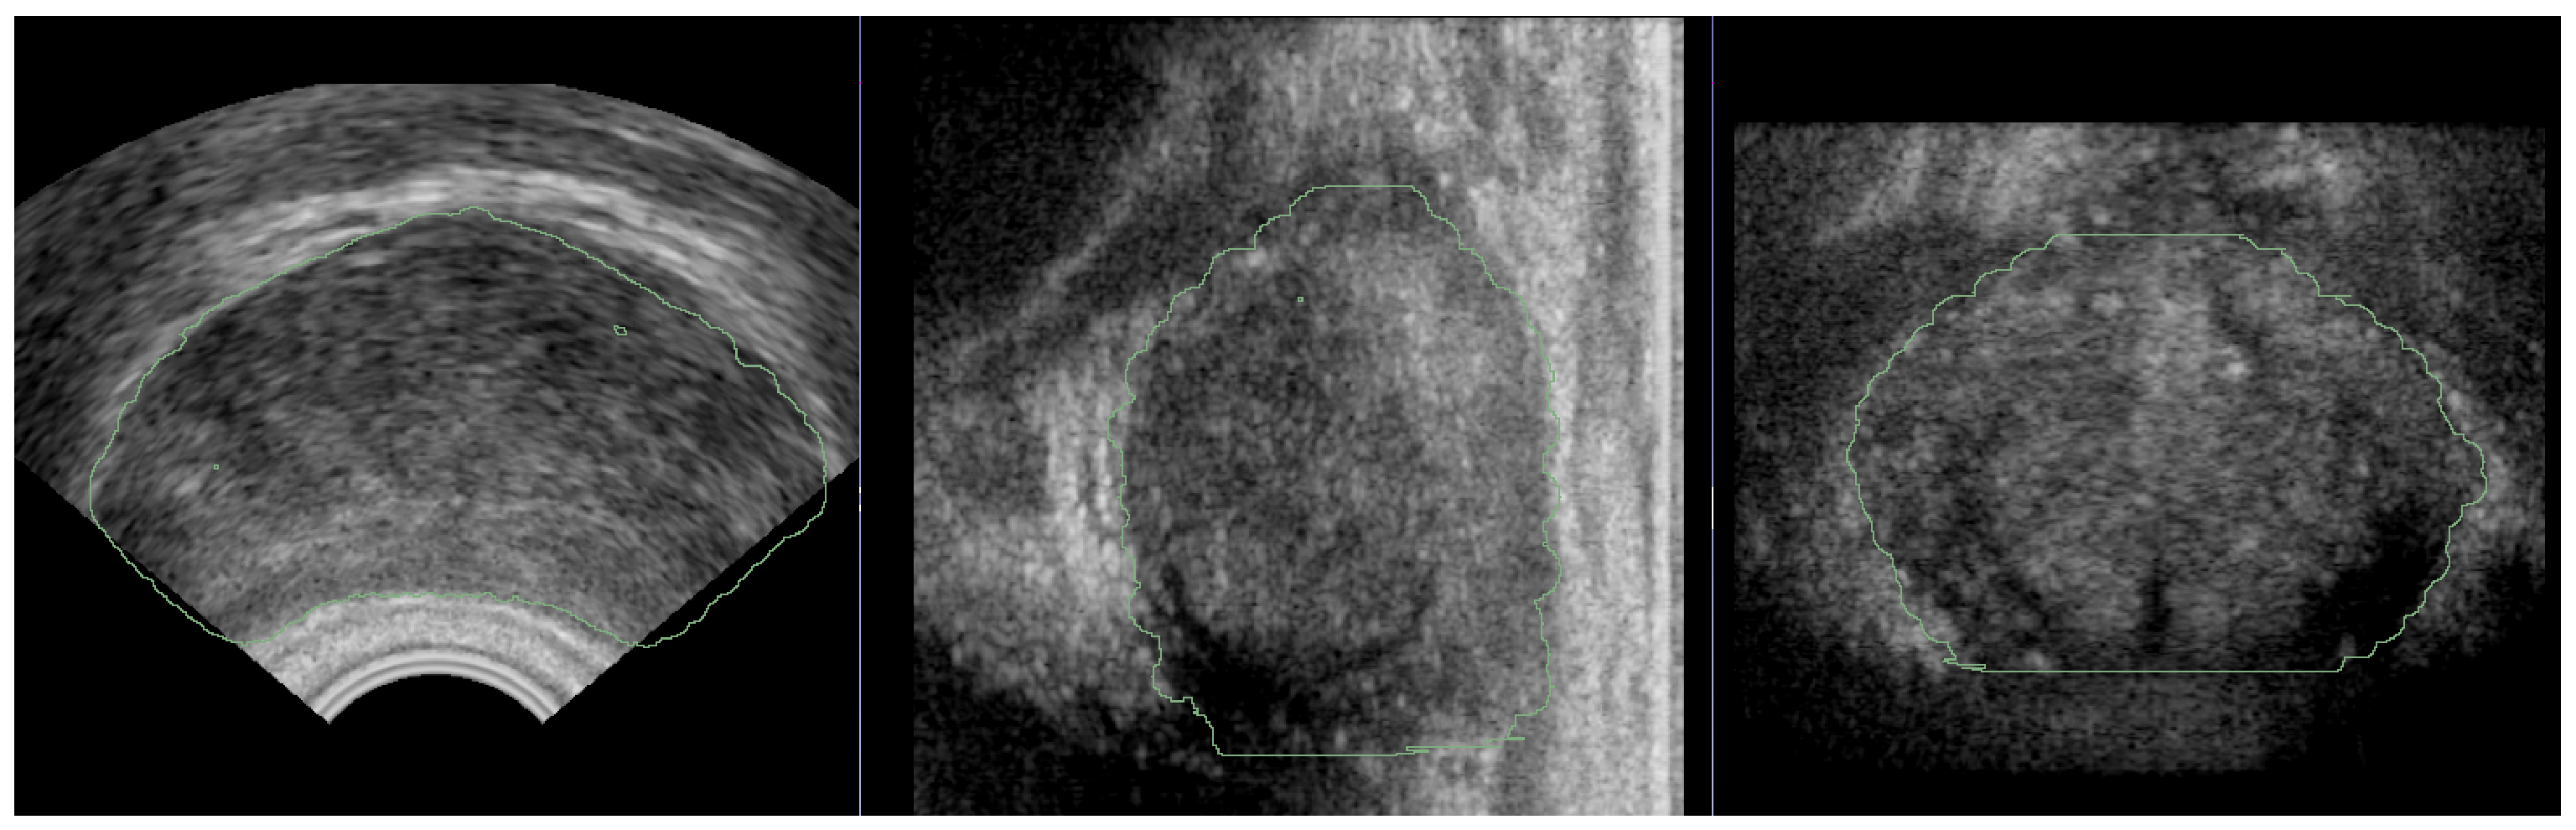
\includegraphics[width=1.0\textwidth]{figs/Bmode_CapsuleSegs.eps} \\
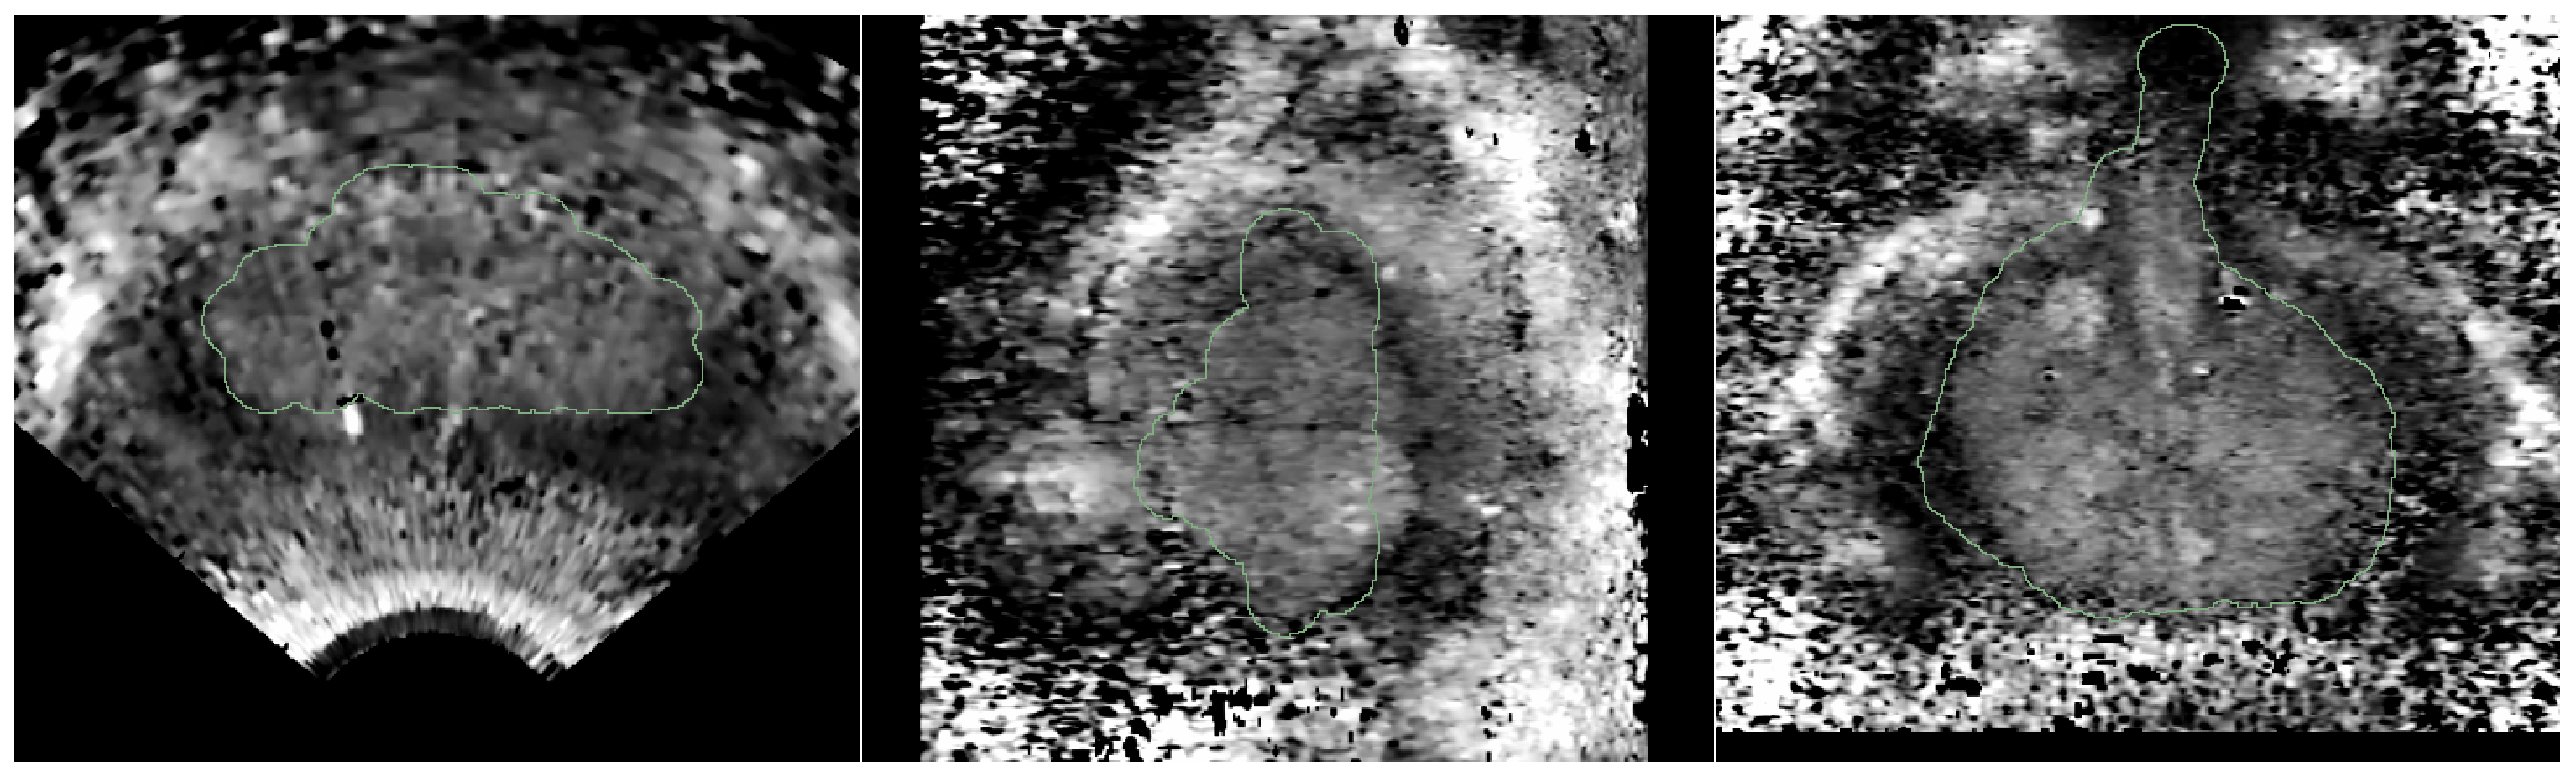
\includegraphics[width=1.0\textwidth]{figs/ARFI_CGsegs.eps} \\
\end{tabular}
\caption{Representative B-mode (top row) and ARFI images (bottom row), with
    superimposed segmentation outlines of the capsule and CG, respectively, for
    the same study subject shown in Figure~\ref{fig:mr_segs_vol}.  The B-mode
    images were segmented in the axial view, using the hypoechoic border of the
    capsule.  Notice that for large prostates, like the one shown in this
    figure, that the edges of the organ were not always captured in the imaging
    field-of-view.  The CG in the ARFI images was typically segmented using the
    coronal view, which, especially in the presence of extensive BPH, can have
    a very characteristic, heterogeneous appearance.  It should be noted that
    the coronal views in these ultrasound images are flipped 180\degree relative
    to the same images in Figure~\ref{fig:mr_segs_vol}.}
\label{fig:arfi_segs} 
\end{figure}
